

\section{Web scraper}

Após uma reunião com o cliente foi compreendido que o catálogo de produtos Motorline não se encontra num servidor. Estes dados apenas estão diretamente no \textit{website} da empresa, sendo assim, foi determinado a necessidade de criar um \textit{web scraper}.

Durante a reunião concluiu-se que o \textit{web scraper} iria apenas correr uma vez por mês para ser evitada a sobrelotação do servidor. Para agilizar a realização do \textit{web scraper} foi entregue pela empresa a estrutura do \textit{website} a seguir para serem obtidas as informações.

\subsection{Implemenção web scraper}
A implementação e testagem do \textit{web scraper}, sem sobrelotação do servidor, foi alcançada, uma vez que, préviamente foi descarregado todo o \textit{wesite} localmente, o que permitiu simular o catálogo.

Para a implementação do \textit{web scraper} optou-se por uma abordagem mais simples. Esta abordagem, consiste na realização de um pedido para ser obtida a página \textit{web}, ler e guardar os dados.

A linguagem utilizada foi \textit{python} devido à facilidade de lidar com abundantes quantidades de dados. O tratamento dos dados das páginas \textit{web} foi realizado com o auxílio da biblioteca \textit{bs4}, também conhecida como \textit{beautiful soup}, esta permite alimentar com uma página \textit{web} e de seguida realizar pesquisas sobre esta com base em \textit{tags} e atributos dos elementos.

Após um estudo do catálogo foi compreendido que dados seriam necessários, sendo estes:
\begin{enumerate}
  \item Categorias e subcategorias de produtos;
  \item Produtos de cada categoria e subcategoria;
  \item Documentação dos produtos;
  \item Imagens e vídeos dos produtos;
\end{enumerate}

\newpage

Para guardar estes dados foi utilizado um dicionário, que contém como chaves as categorias de produtos. Para cada categoria contém mais um dicionário com as subcategorias de produtos. Cada categoria possui uma lista de produtos, sendo cada produto representado por um dicionário, que abarca como chaves os seus atributos.
A utilização de dicionários e listas para guardar estes dados deve-se a que o objetivo será guardar estes em \textit{json} e a transformação é simplificada com a utilização destas estruturas devido à proximidade com a estrutura \textit{json}.

\begin{figure}[htb]
  \centering
  
  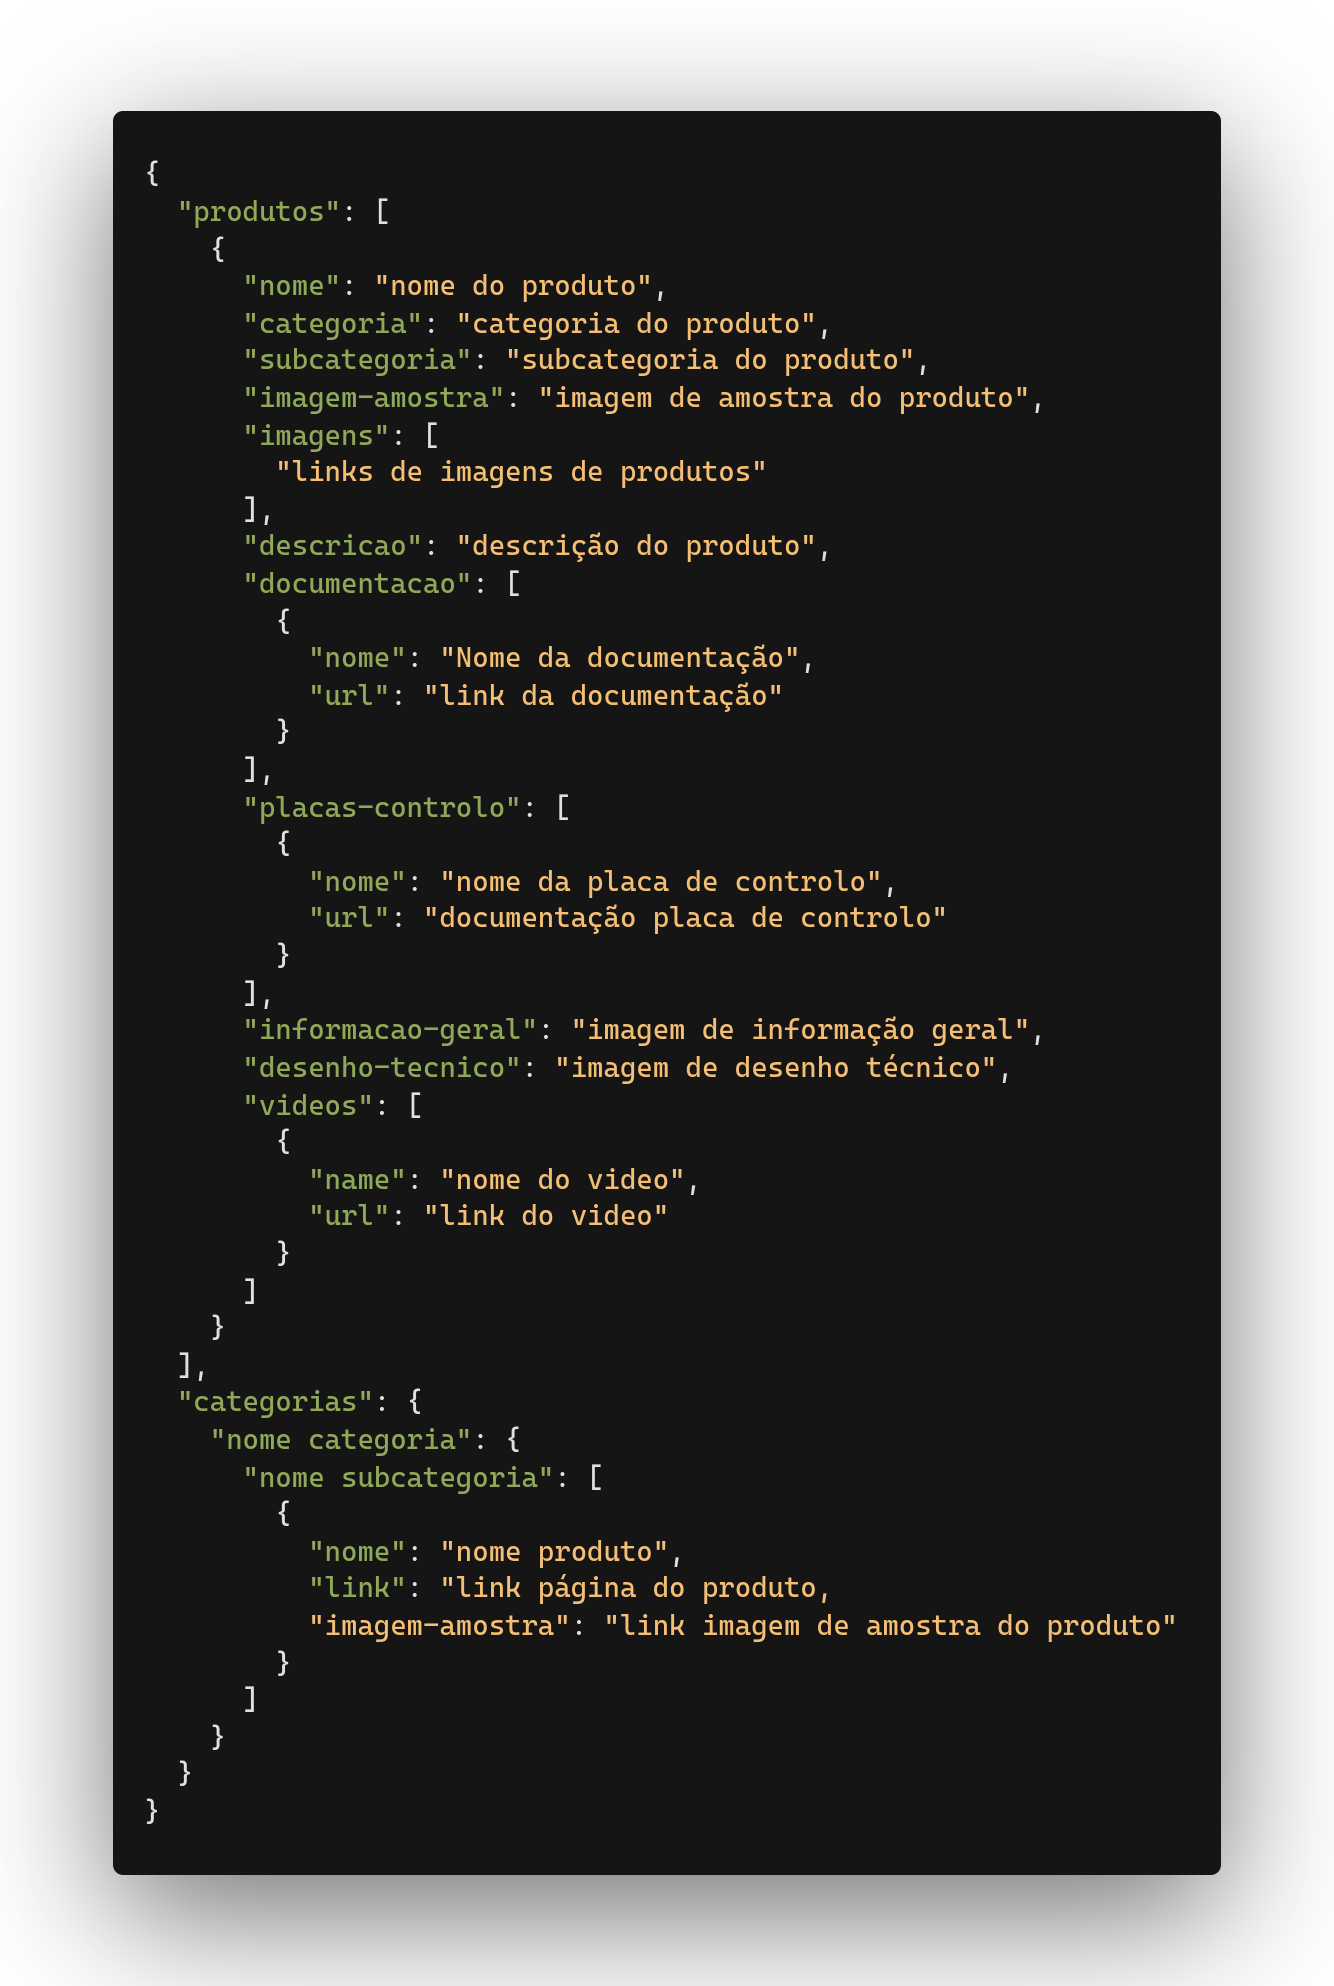
\includegraphics[width=0.7\textwidth]{images/implementacao/scraper/estrutura_scraper.png}
  \caption{Estrutura dos dados obtidos}
  \label{fig:49}
\end{figure}

\newpage

Após uma análise da estrutura do \textit{website} foi constatado que a página geral dos produtos possui todas as categorias, assim como, as subcategorias com \textit{urls} para as páginas que contém todos os produtos das subcategorias. 

Sendo assim, em primeiro lugar percebeu-se que cada conjunto(categoria, subcategorias) é uma secção, pelo que, são obtidas todas as secções das categorias. Para cada uma destas secções, é obtido o título que equivale ao nome da categoria e também todos os elementos clicáveis. Estes, correspondem às subcategorias que contêm o nome e um \textit{url}, que redireciona para a página de produtos da subcategoria.

\begin{figure}[htb]
  \centering
  
  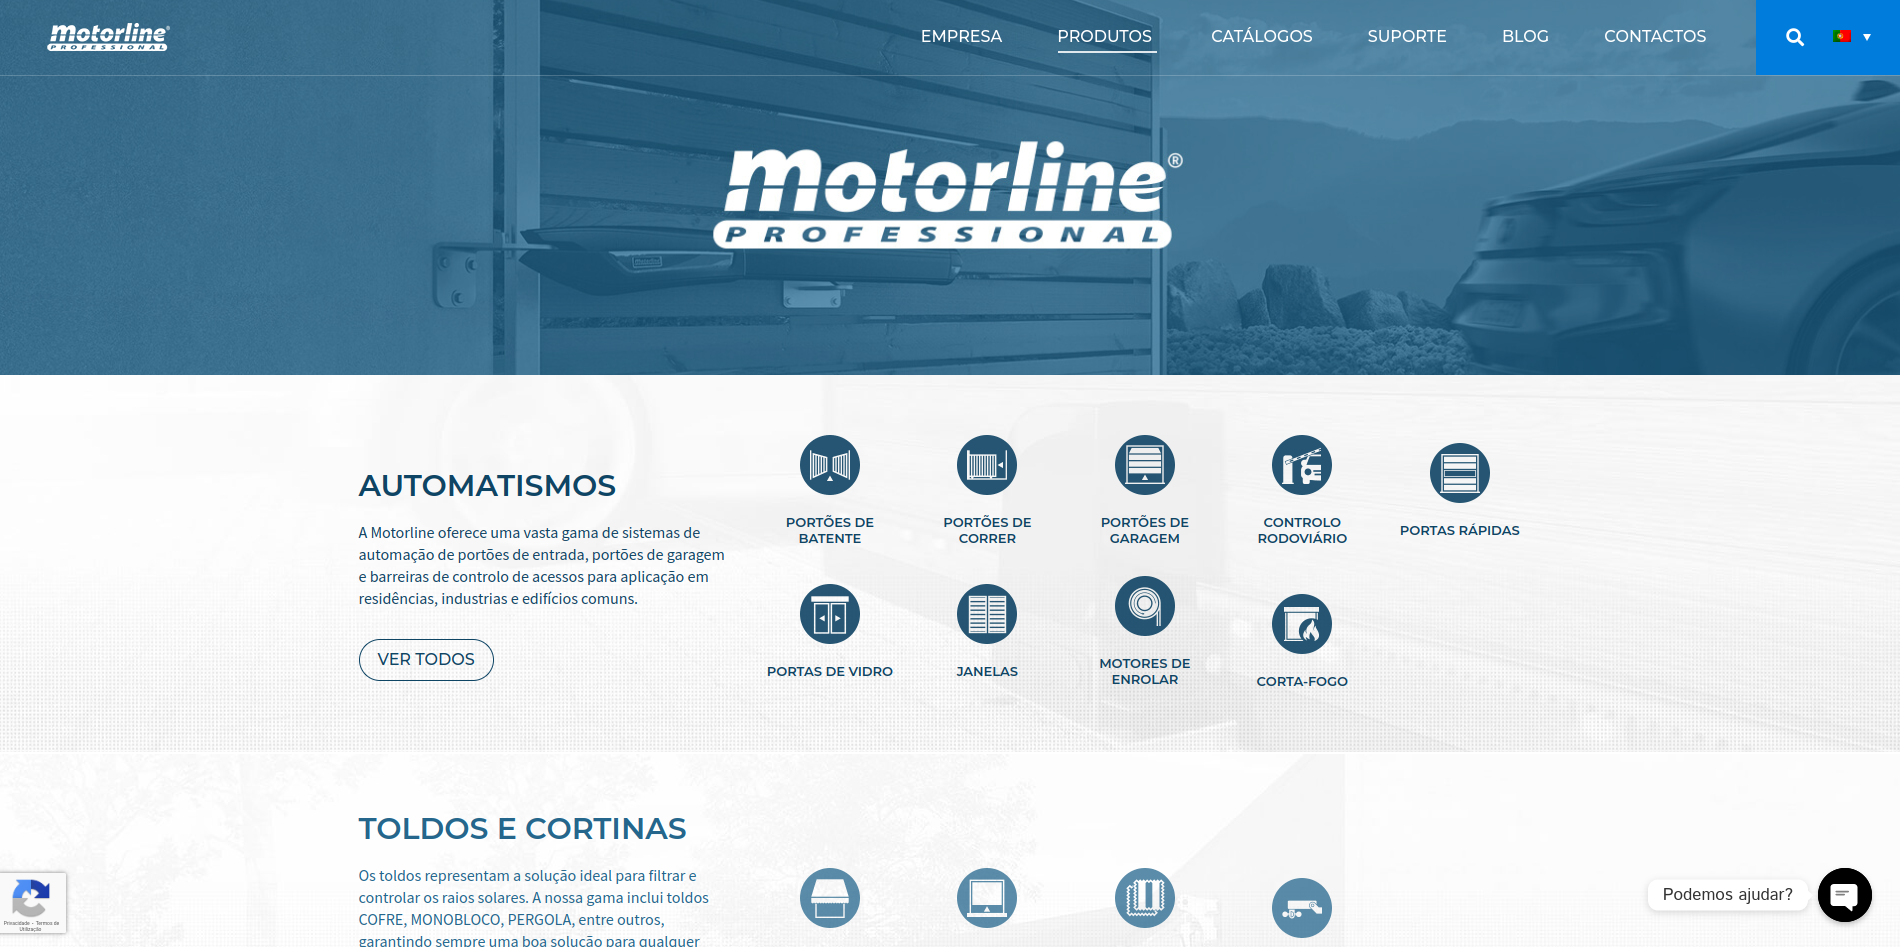
\includegraphics[width=0.55\textwidth]{images/implementacao/scraper/pagina_geral_produtos.png}
  \caption{Página geral de produtos}
  \label{fig:50}
\end{figure}

Posto isto, já é possível identificar cada categoria e subcategoria, assim como, o \textit{url} da página de produtos para cada subcategoria. Mas, após alguma análise dos dados foi percebido que estas não contêm acentuação visto que, existe uma formatação no \textit{website}. Para resolver este problema, foram pesquisadas ferramentas capazes de corrigir erros ortográficos. Pelo que, descobriu-se que a biblioteca mais utilizada em \textit{python} para resolver este problema é a biblioteca \textit{spellchecker}. Esta ferramenta, por sua vez, é a mais utilizada dado à sua capacidade de correção dos erros ortográficos em diversas linguagens. Por fim, sempre que uma categoria e subcategoria é obtida, antes de ser guardada, é corrigida.


Aquando a finalização do processo anterior, cada \textit{url} é aberto e a partir disto, são obtidos os \textit{urls} de produtos e imagens de amostra dos produtos. Em cada página, foram obtidos todos os elementos pressionáveis existentes, sendo que cada um refere-se a um produto. Para obter o nome do produto correspondente, foi utilizado o nome contido no \textit{url} do elemento, pois todos os produtos seguem a mesma estrutura, sendo esta, /produtos/nome-produto. Como em \textit{urls} não é permitido utilizar acentuação e espaços, todos os nomes foram corrigidos com a mesma ferramenta de correção ortográfica mencionada anteriormente.

\begin{figure}[htb]
  \centering
  
  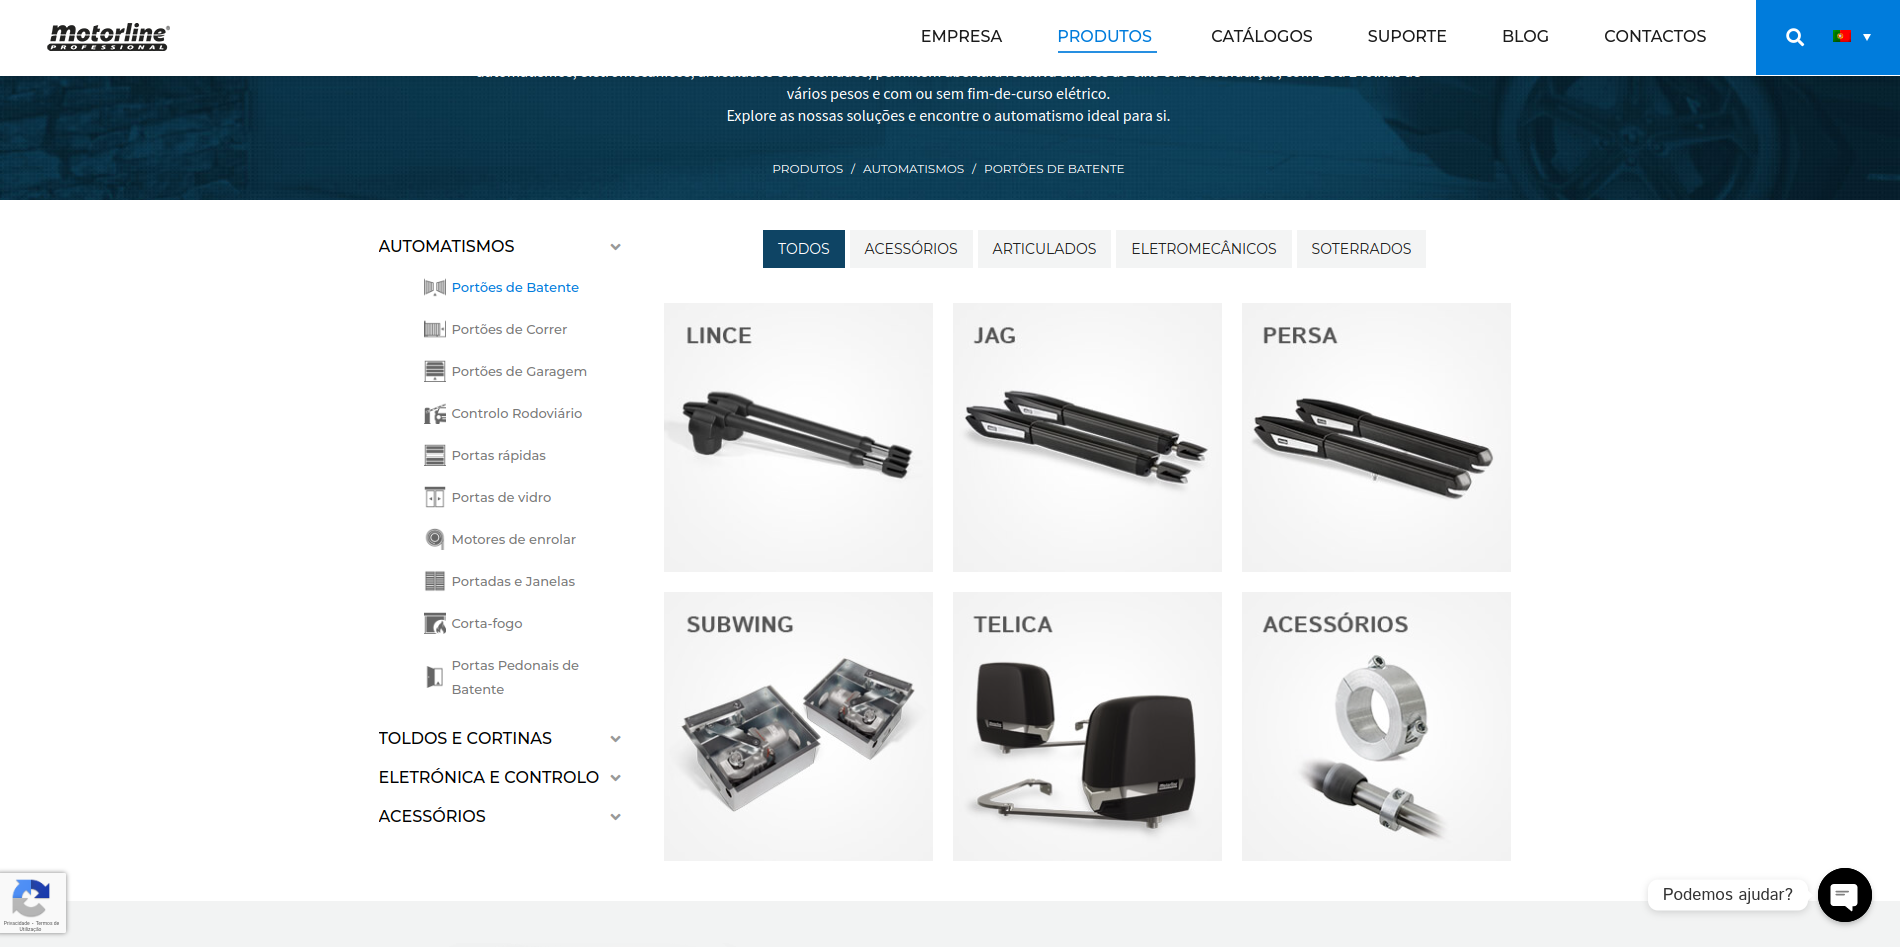
\includegraphics[width=0.55\textwidth]{images/implementacao/scraper/pagina_produtos_subcat.png}
  \caption{Página de produtos de uma subcategoria}
  \label{fig:51}
\end{figure}

\newpage
Neste momento, depois de correr o código foi deduzido que existem algumas páginas de produtos em que este não conseguia obter dados, pelo que, um erro era atirado. Para compreender exatamente em que páginas de produtos surgia este erro, sempre que um erro era detetado, este \textit{url} era adicionado a uma nova chave do dicionário mencionado anteriormente. Esta chave, tem o nome \textit{misses} e contém todos os \textit{urls} em que algum erro aconteceu. Então, nesta ocasião percebeu-se que nem todas as páginas de produtos são iguais, contudo, após uma reunião com o cliente este expôs que existem páginas de produtos e de detalhes de produtos que são muito diferentes das restantes.

\begin{figure}[htb]
  \centering
  
  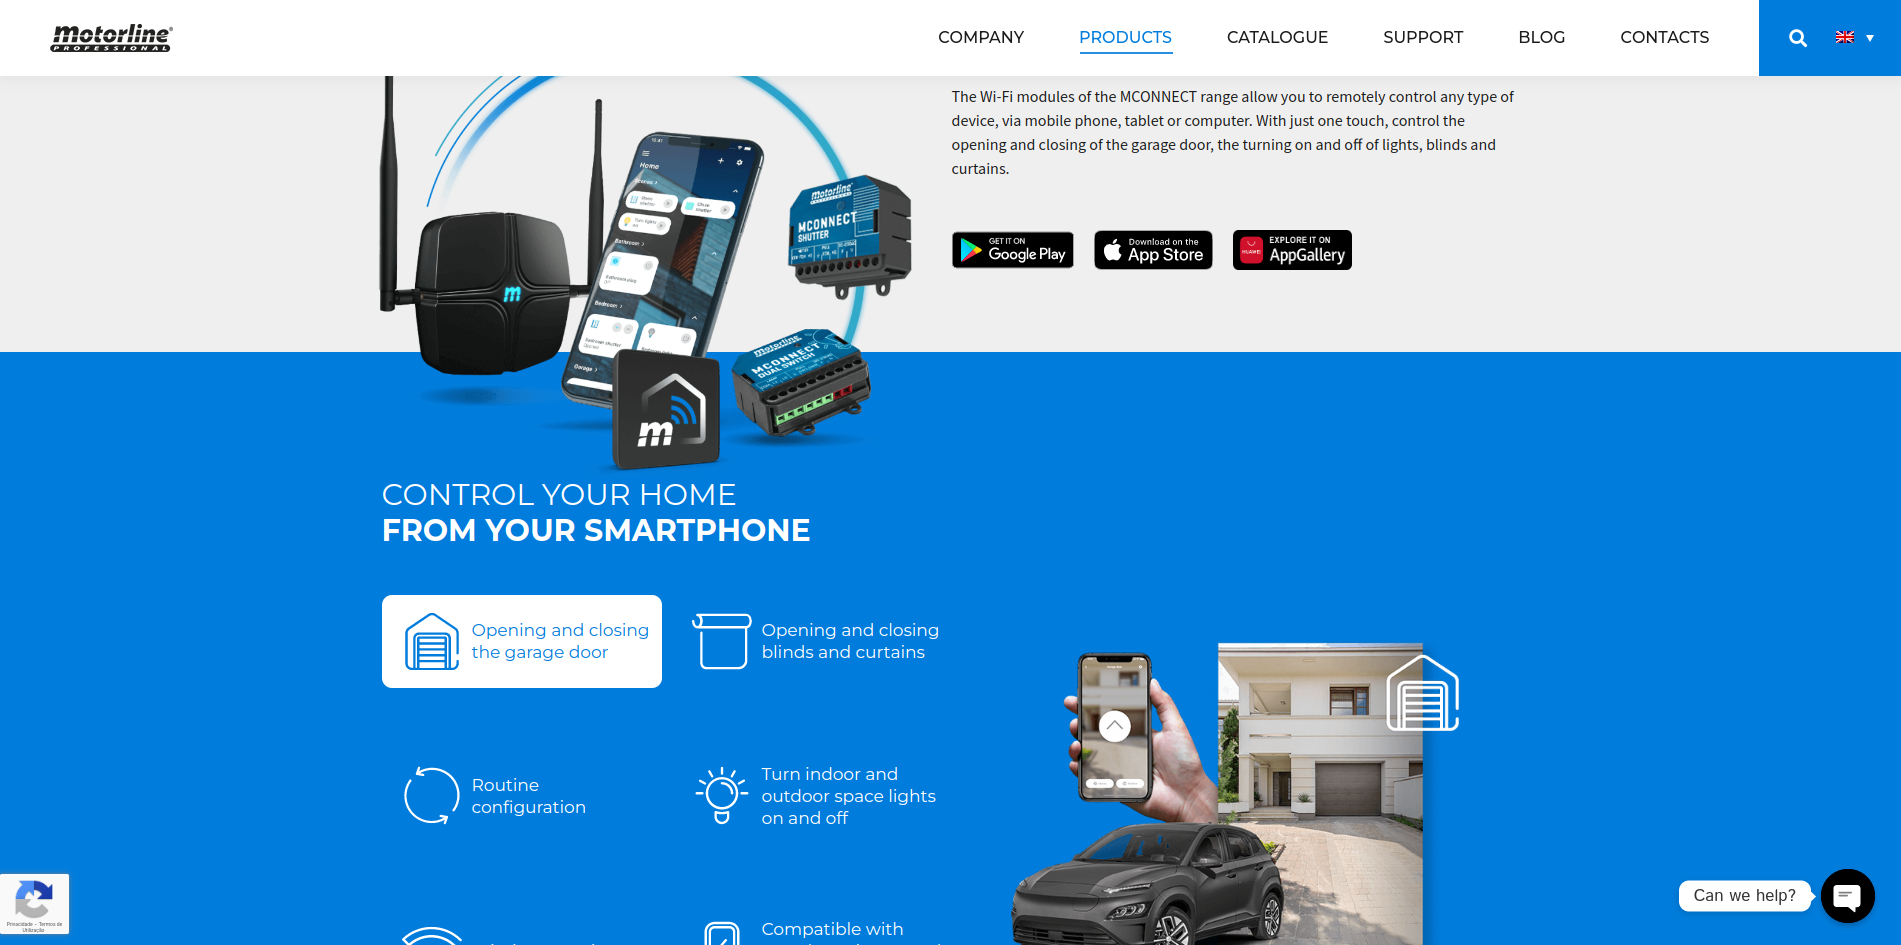
\includegraphics[width=0.7\textwidth]{images/implementacao/scraper/mconnect.png}
  \caption{Página de produtos de uma subcategoria distinta}
  \label{fig:52}
\end{figure}

Com o objetivo de não atrasar o restante projeto foi determinado primeiramente, que todos os produtos que contêm páginas semelhantes deveriam ser obtidos. Para cada página de produto, foi obtido o título que corresponde ao nome do produto e o elemento que contém o \textit{id} produto-descrição, que corresponde à sua descrição. As imagens dos produtos são disponibilizadas através de \textit{urls} na secção da galeria do produto, pelo que, são obtidos todos os seus \textit{urls}.

A documentação dos produtos pode ser disponibilizada através de \textit{urls} para os manuais, ou, com uma lista \textit{dropdown} com todos os manuais em formato \textit{url}, o que permite, serem obtidos através de todos os \textit{urls} da secção de documentação, assim como, os nomes e todas as opções do \textit{dropdown} se este existir.

\begin{figure}[htb]
  \centering
  
  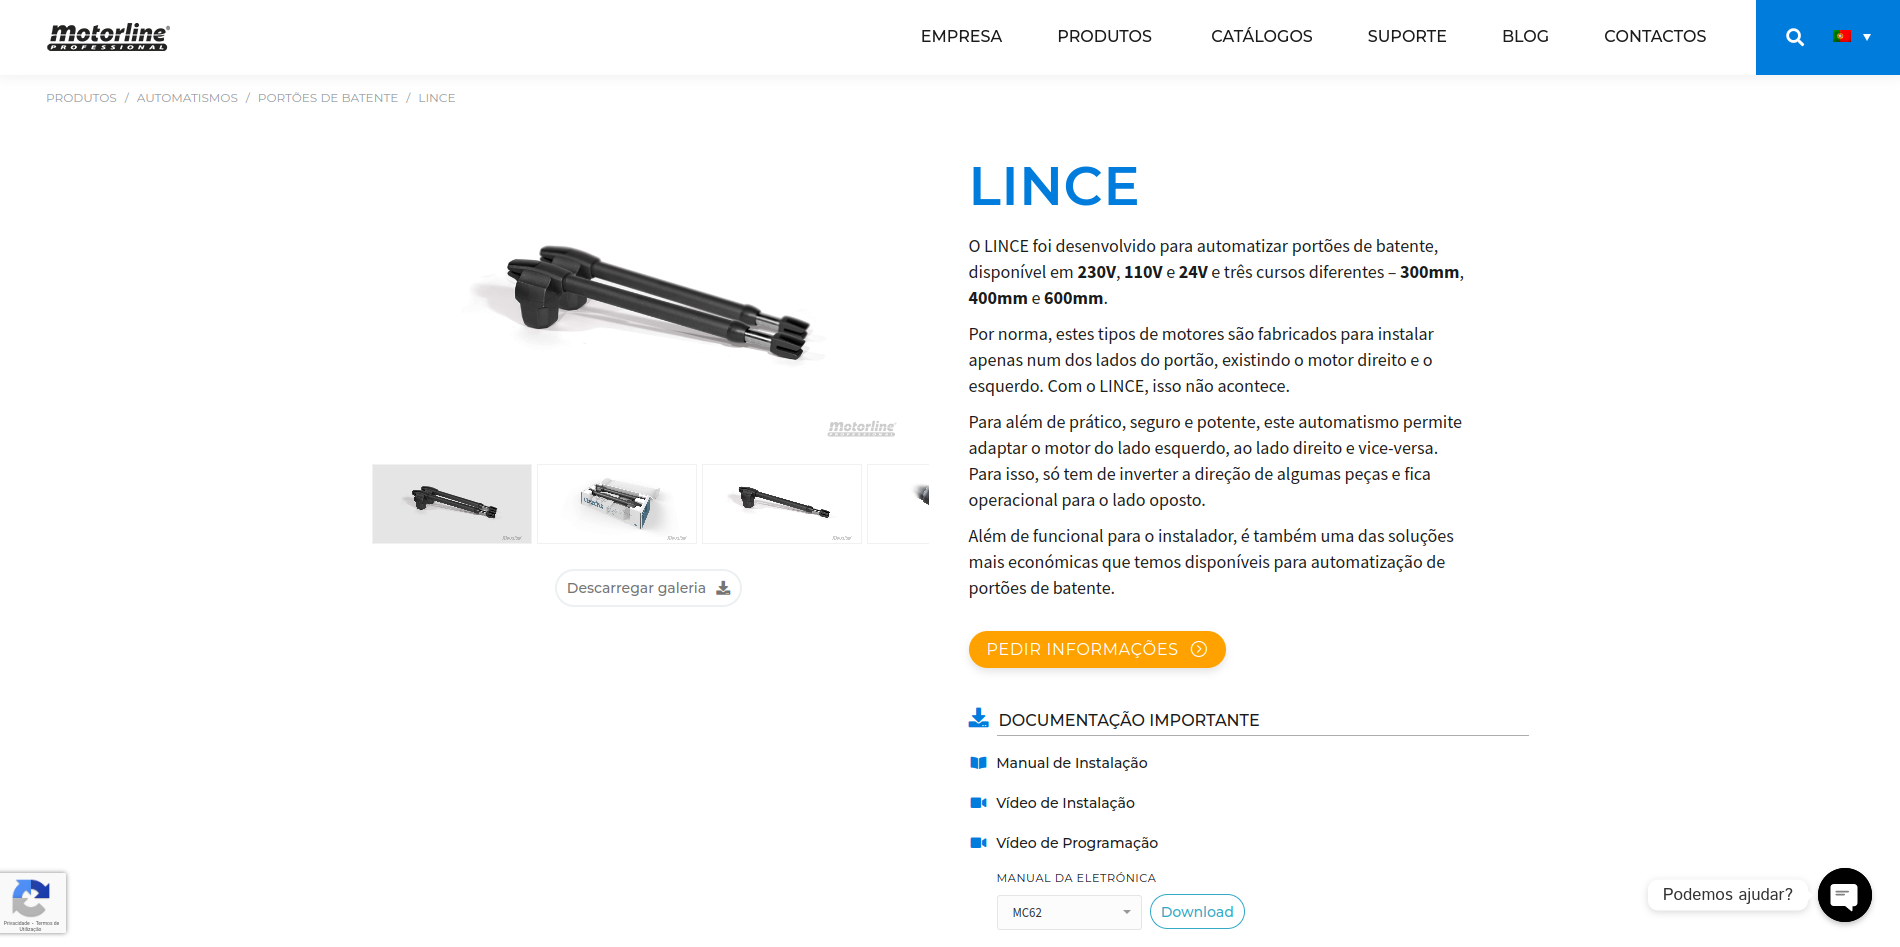
\includegraphics[width=0.7\textwidth]{images/implementacao/scraper/pagina_detalhes_produto.png}
  \caption{Página de detalhes de produto, secção inicial}
  \label{fig:53}
\end{figure}

\newpage

As imagens de desenho técnico e informação geral encontram-se disponíveis na secção correspondente ao nome de cada uma, caso existam, são obtidas as imagens e os seus \textit{urls}.

\begin{figure}[htb]
  \centering
  
  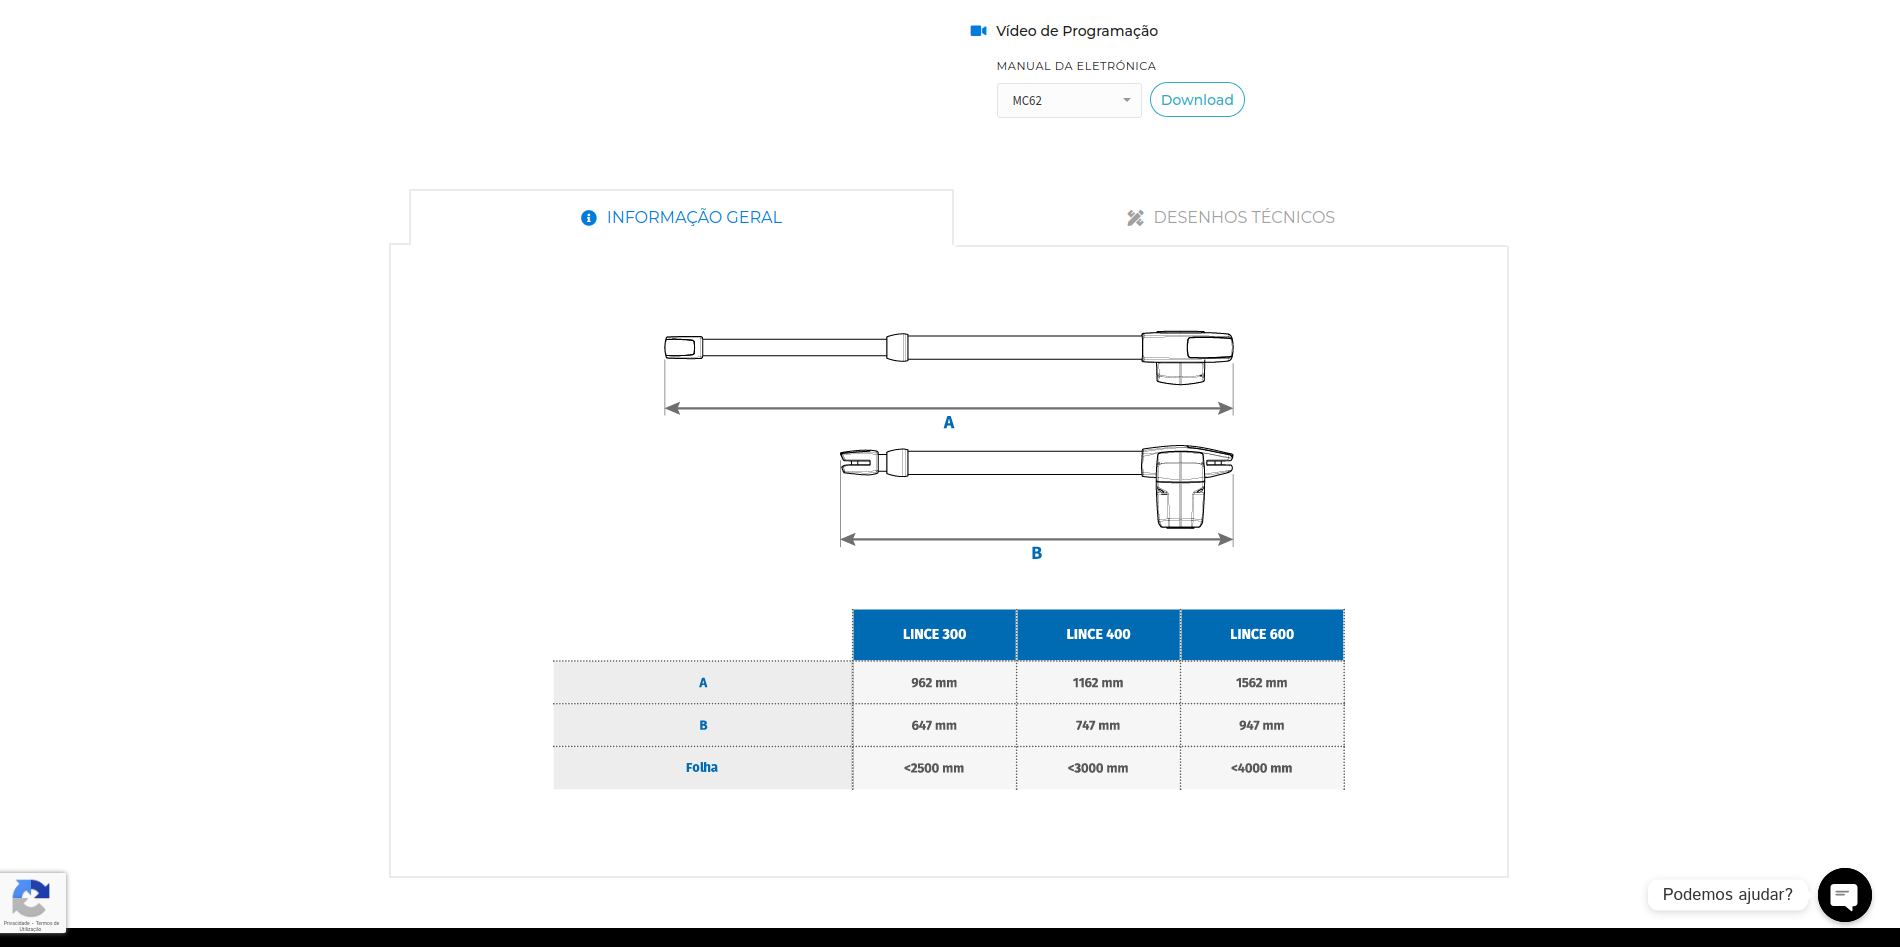
\includegraphics[width=0.7\textwidth]{images/implementacao/scraper/pagina_detalhes_desenhos.png}
  \caption{Página de detalhes de produto, secção de informações}
  \label{fig:54}
\end{figure}

Os vídeos de produtos estão disponíveis na secção de vídeos, sendo que, cada uma contém o nome e o vídeo. Estes são demonstrados através da utilização de um elemento \textit{iframe}, este contém um \textit{url} para o vídeo, mas após a tentativa de visualização deste \textit{url}, constatou-se que não é possível obter o vídeo a partir deste. Sendo assim, foi investigada a plataforma \textit{vimeo}. Esta, contém todos os vídeos de produtos, pelo que, para cada um é gerado um \textit{id} único. Este vídeo poderá ser acedido através do \textit{url} geral da plataforma seguido do \textit{id}. O \textit{id}, está colocado no elemento \textit{iframe}, pelo que, é obtido e acrescentado ao \textit{url} da plataforma, o que permite guardar todos os vídeos de produtos.

\begin{figure}[htb]
  \centering
  
  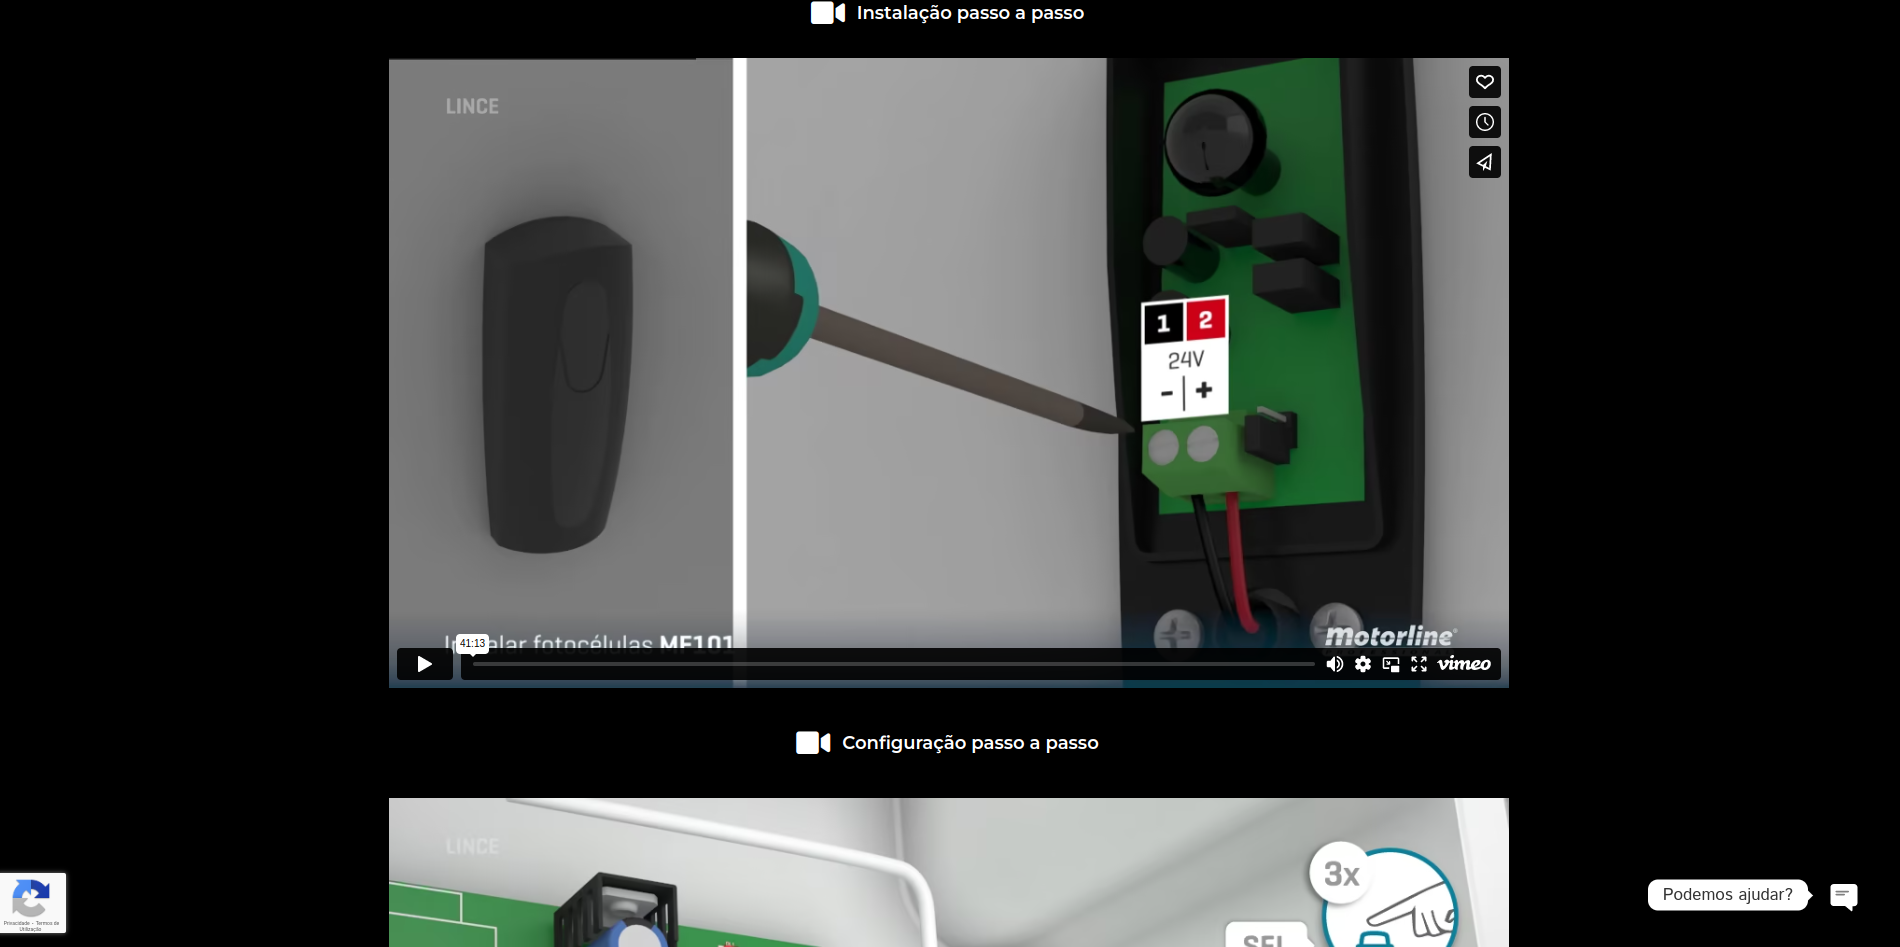
\includegraphics[width=0.7\textwidth]{images/implementacao/scraper/pagina_detalhes_videos.png}
  \caption{Página de detalhes de produto, secção de videos}
  \label{fig:55}
\end{figure}

\newpage

\subsubsection{Implemenção no website}

Logo que se verificou que pelo menos 80\% dos produtos totais eram obtidos, decidiu-se testar no \textit{website}. Para isto, foi utilizada a biblioteca \textit{requests}, com a qual é realizado um pedido \textit{GET} a cada \textit{url} necessário para obter a página \textit{web}. Assim que o código foi corrido e a resposta analisada compreendeu-se que o \textit{website} bloqueia este tipo de solução como é indicado na figura~\ref{fig:56}

\begin{figure}[htb]
  \centering
  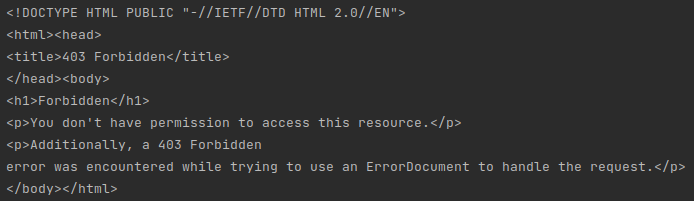
\includegraphics[width=0.7\textwidth]{images/implementacao/scraper/forbiden_response.png}
  \caption{Resposta obtida aquando o pedido ao \textit{url} da página \textit{web}}
  \label{fig:56}
\end{figure}

Através da resposta obtida, foi compreendida a necessidade de alteração da abordagem, visto que, a anterior não poderia ser utilizada. Opcionalmente seria possível seguir a abordagem de simular a ação humana através da abertura de um navegador programáticamente e pesquisar pelo \textit{url} desejado. 

Após uma investigação descobriu-se que existem ferramentas que permitem controlar o dispositivo onde correm, mas estas impedem a utilização enquanto se encontram a correr. Também, foram descobertas ferramentas que apenas recebem o navegador a utilizar e abrem uma nova janela deste para realizar a pesquisa.
O processo de obter os produtos é demorado, pelo que, optou-se pela segunda opção, uma vez que, seria possível continuar com o trabalho em paralelo com o processo de obter dados. Sendo assim, a ferramenta mais recomendada para realizar esta operação é a biblioteca \textit{selenium}.

Com a utilização da biblioteca \textit{selenium} indicou-se qual o navegador a utilizar. Neste caso foi escolhido o \textit{chrome}, dado que, encontrava-se instalado no dispositivo. Após ser indicado qual o navegador a utilizar, é necessário para cada página referir qual o elemento a esperar que carregue, pois, por vezes existem elementos que demoram mais tempo a carregar do que a página. A página carregada poderá não conter o elemento a obter, pelo que foi implementado um tempo de espera máximo de 5 segundos, assim que este tempo expira, a operação é cancelada e o \textit{url} é adicionado à lista de \textit{urls} com erros.

\newpage


\subsubsection{Melhoria de implementação}

Depois de completo o processo, foi decidido melhorar a implementação com a resolução dos erros encontrados em \textit{urls} específicos. Para perceber exatamente quais os \textit{urls} que possuem erros, foram direcionados os dados obtidos para um ficheiro \textit{json}. Sendo assim, os \textit{urls} com erros eram os indicados na figura~\ref{fig:57}.

\begin{figure}[htb]
  \centering
  
  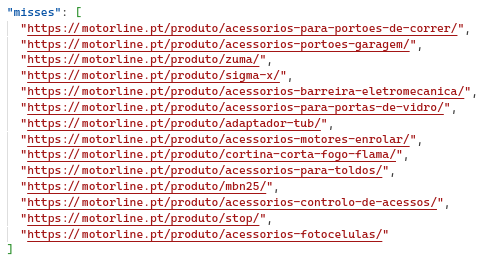
\includegraphics[width=0.7\textwidth]{images/implementacao/scraper/urls_erro_iteracao_1.png}
  \caption{Urls com erro primeira interação}
  \label{fig:57}
\end{figure}

Posteriormente a uma primeira análise percebeu-se que grande maioria os erros provêm de \textit{urls} de acessórios de produtos, isto deve-se ao facto destes encontrarem-se na página de produtos de subcategoria e serem tratados como um produto, sendo assim, sempre que se trata de um url de acessórios seria necessário correr código para obter dados de acessórios ao invés de detalhes de produtos. Deste modo, compreendeu-se que nos \textit{urls} a palavra accessórios está sempre contida, o que permite que sempre que esta é detetada num \textit{url}, seja corrido o código referente a obter de acessórios. Para desenvolver este código foi primeiramente analisada a página de acessórios de produtos(Figura~\ref*{fig:58}), esta contém para cada acessório um elemento do tipo artigo o qual detém uma imagem, titulo e descrição. Esta descrição por vezes possui \textit{urls} para os produtos aos quais este acessório se refere. Sempre que estes \textit{urls} são detetados, os nomes dos produtos são guardados para futuramente realizar a ligação entre os acessórios e os produtos, dado que, não existem produtos com nomes iguais. 

\begin{figure}[htb]
  \centering
  
  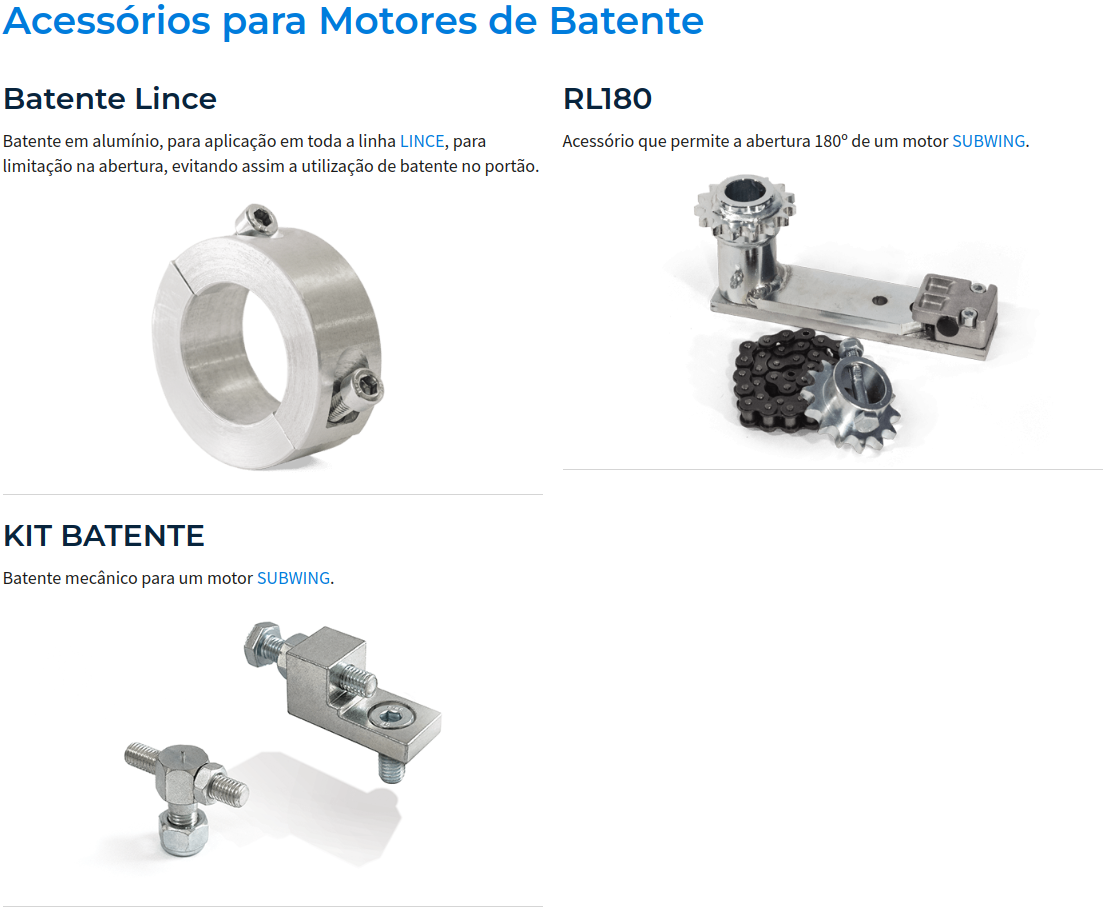
\includegraphics[width=0.45\textwidth]{images/implementacao/scraper/pagina_acessorios.png}
  \caption{Exemplo de página de acessórios}
  \label{fig:58}
\end{figure}

\newpage

Na iteração seguinte determinou-se que a quantidade de \textit{urls} com erros diminuiu, mas mesmo assim existiam produtos com erro, pelo que, estes foram analisados e percebeu-se que o erro ocorria, visto que, por vezes as páginas não continham os vídeos ou imagens de documentação. Para resolver este problema, o código foi alterado para somente obter estes dados se os elementos existirem na página. Após correr novamente o código foi compreendido que a quantidade de falhas obtidas diminuiu drasticamente (Figura~\ref{fig:59}), mas mesmo assim, ainda existiam quatro falhas a ocorrer e após uma análise foi determinado que estas ocorriam devido a uma página de subcategoria de produtos conter um serviço, um produto conter uma página de detalhes de produto com sub produtos, existir uma página de adaptadores de produtos e um produto conter uma página de detalhes diferente das demais.

% \begin{enumerate}
%   \item Uma página de subcategoria de produtos conter um serviço;
%   \item Um produto conter uma página de detalhes de produto com sub produtos;
%   \item Existir uma página de adaptadores de produtos;
%   \item Um produto conter uma página de detalhes diferente das demais;
% \end{enumerate}

\begin{figure}[htb]
  \centering
  
  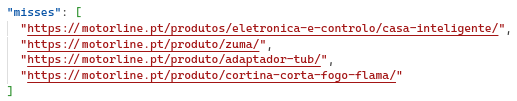
\includegraphics[width=0.7\textwidth]{images/implementacao/scraper/melhor_corrida.png}
  \caption{Indicação das páginas com falha}
  \label{fig:59}
\end{figure}



A página de adaptadores de produtos segue uma estrutura similar à dos acessórios, pelo que foi a primeira a ser abordada e resolvida através do código de obter detalhes de acessórios. Neste sentido este foi alterado para executar sempre que a palavra acessórios ou adaptadores encontra-se no \textit{url}.

A resolução do problema de existirem serviços e subprodutos implica uma alteração no diagrama de entidade relação, pelo que, o problema do produto que contém uma página de detalhes diferente das demais foi resolvido primeiro. Este produto para além da dificuldade de ser uma página completamente diferente, as informações encontram-se espalhadas (Figura~\ref*{fig:60}), o que leva a que estas tenham de ser combinadas para construir os detalhes do produto. Após obter-se estes dados foi determinado que as imagens do produto têm dados escritos que não se encontram na imagem original. Para a solução deste problema o cliente recomendou obter com \textit{screenshots} e guardar num servidor de imagens.

\begin{figure}[htb]
  \centering
  
\includegraphics[width=0.7\textwidth]{images/implementacao/scraper/flama.png}
  \caption{Exemplo de página de produto incomum}
  \label{fig:60}
\end{figure}

\newpage

O problema de existirem produtos com subprodutos foi resolvido através da alteração da base de dados, à qual foi adicionada uma nova ligação sobre si mesma na tabela produtos, o que permite que um subproduto possua uma ligação com produto principal. Após ser feita esta alteração, o código para obter os dados do catálogo foi alterado. Em primeiro lugar, foram obtidos todos os dados do produto principal e de seguida os dados específicos a cada subproduto, o que leva a que a organização do produto principal seja igual aos restantes, mas, com um dado extra com os subprodutos. 

\begin{figure}[htb]
  \centering
  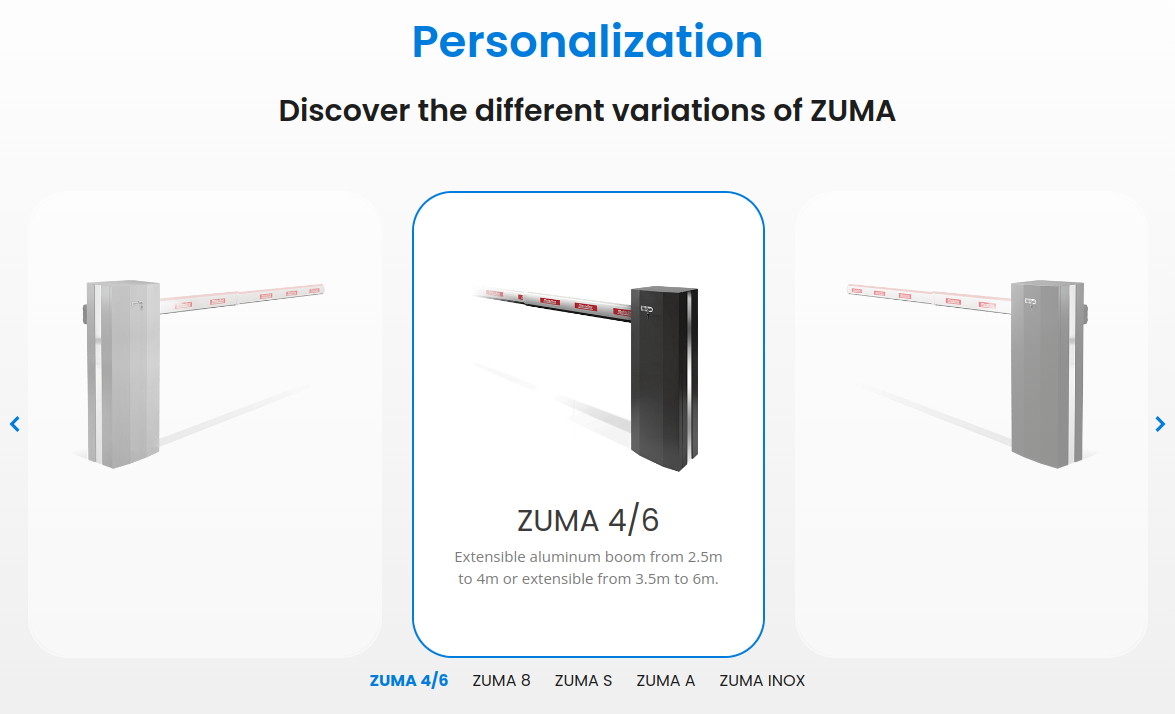
\includegraphics[width=0.6\textwidth]{images/implementacao/scraper/zuma.png}
  \caption{Exemplo de página de produto com subprodutos}
  \label{fig:61}
\end{figure}

O último problema a solucionar é a existência de serviços, pelo que, iniciou-se pela análise deste tipo de produto. Este possui descrição e imagens como os produtos, mas também vídeos direcionados a plataformas diferentes, produtos do serviço, registo de atualizações do serviço, planos de pagamento e cada plano contém diversas ofertas. 
Através da estrutura de um serviço foi adicionado à base de dados as tabelas de serviço, planos do serviço, ofertas dos planos, vídeos do serviço, informações de atualizações dos serviços, imagens do serviço e a ligação à tabela produtos, o que permite a identificação dos produtos do serviço. Aqui, foi identificada a necessidade de manter guardado os \textit{links} para todas as imagens e vídeos na própria base de dados, visto que, existem imagens que não sabem ainda qual é o \textit{id} do produto referente, pelo que não seria possível no futuro obtê-las sem alteração manual, o que levou a que estas tabelas também existam para os produtos. De seguida compreendeu-se que existem dados que não são necessários na descrição, o cliente recomendou guardar estes dados como \textit{screenshots}.
\begin{figure}[htb]
  \centering
  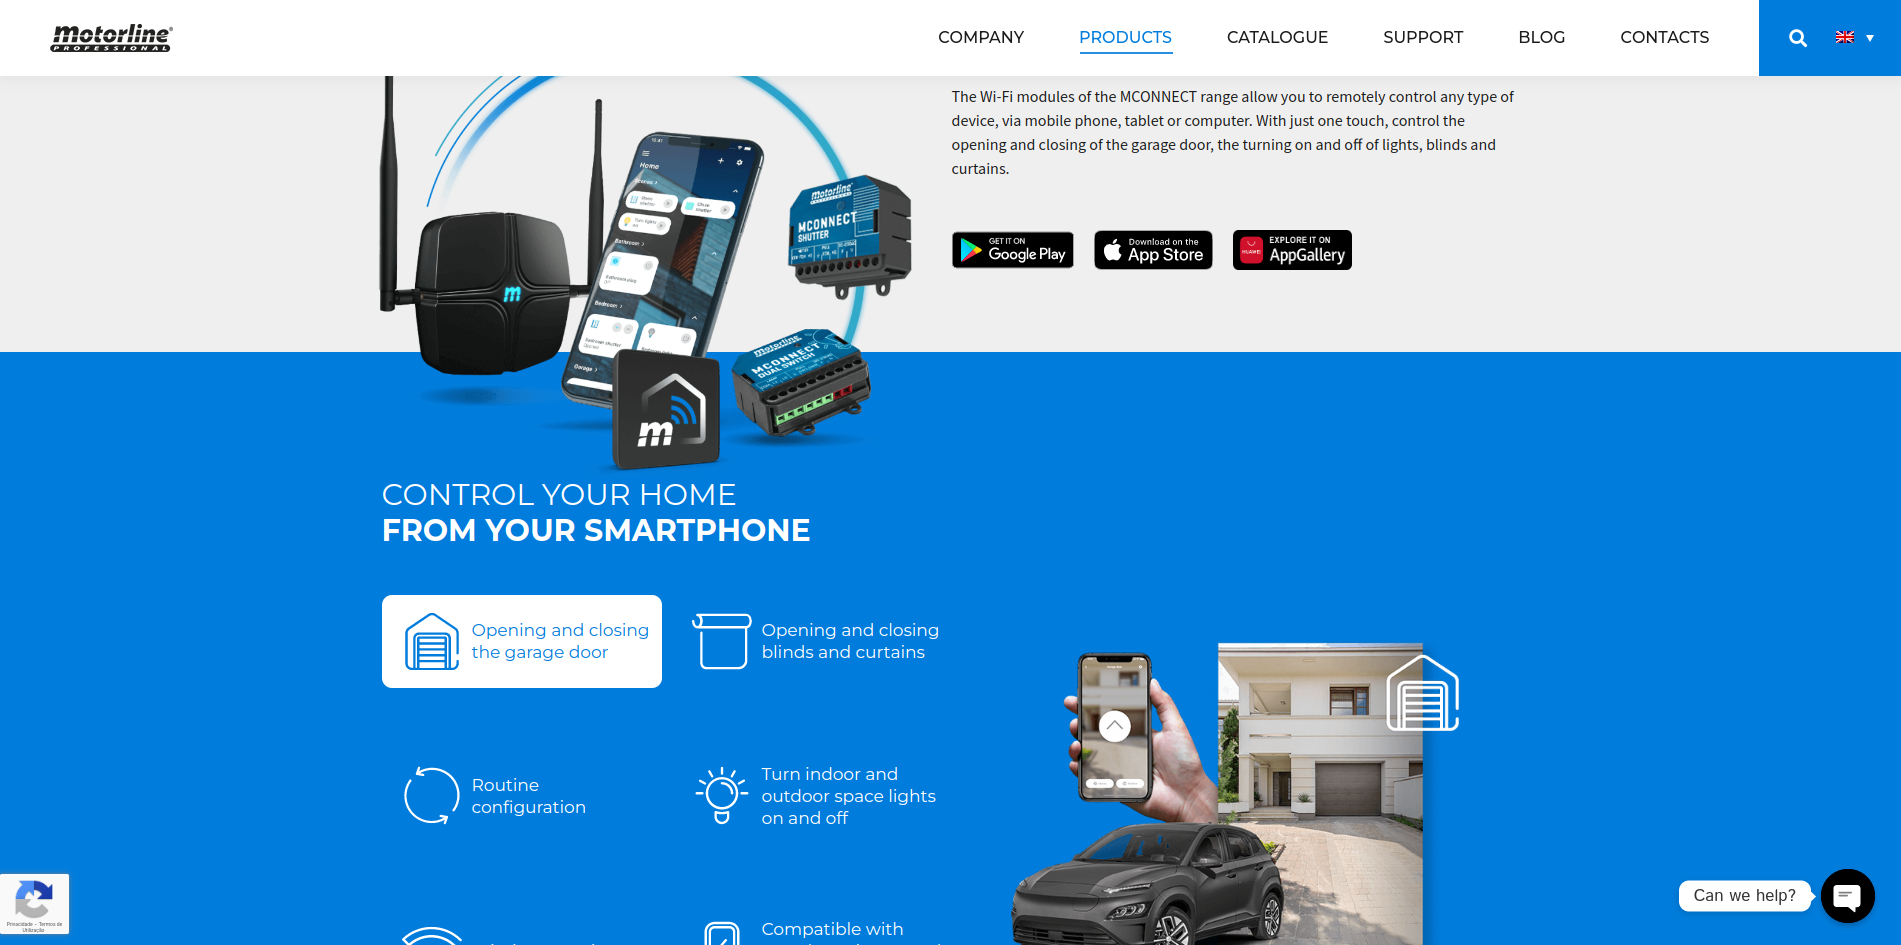
\includegraphics[width=0.6\textwidth]{images/implementacao/scraper/mconnect.png}
  \caption{Exemplo de página de serviço}
  \label{fig:62}
\end{figure}


\subsubsection{Diagrama de base de dados final}

Após as alterações mencionadas à base de dados, o seu diagrama final encontra-se na Figura~\ref{webscraper_bd}

\begin{figure}[htb]
  \centering
  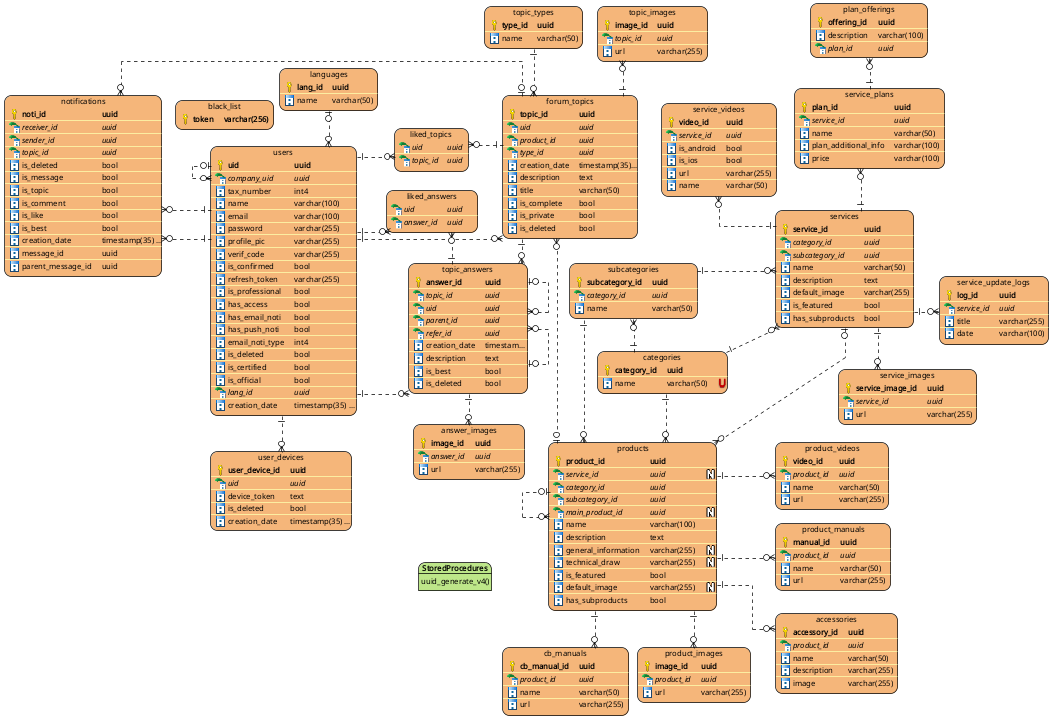
\includegraphics[width=0.9\textwidth]{images/diagramas/bd_final.png}
  \caption{atualização da base de dados}
  \label{webscraper_bd}
\end{figure}


\subsubsection{Armazenamento de dados}

Após obter-se os dados dos produtos, é necessário guardar na base de dados para serem disponibilizados ao \textit{backend}. Para realizar esta operação existiam duas opções, criar um serviço para inserir produtos e realizar um pedido a este serviço, ou então, conectar diretamente o \textit{web scraper} à base de dados. Não seria de grande interesse conectar diretamente à base de dados, pelo que, foi decidido criar um serviço que recebe um produto e o insere. O grande problema que surgiu com esta solução é que os pedidos ocorrem de forma sequencial, mas com pouco tempo de espera, o que levou a que o limite máximo de conexões com a base de dados fosse extrapolada. Isto acontece porque para cada serviço que recebe uma chamada é desenvolvida uma nova conexão à base de dados, todas as operações são realizadas e por fim a conexão é terminada, mas enquanto estas operações estão a decorrer, o servidor poderá receber mais pedidos, o que leva a que mais conexões sejam criadas, o que atinge assim rápidamente o limite de conexões da base de dados. Como solução para este problema foi acrescentado uma espera de 0.5 segundos a cada pedido. A inserção de serviços decorreu com o mesmo processo.

A inserção de categorias decorre através do envio das categorias a inserir num \textit{array}, o que leva a que estas sejam inseridas todas num pedido. As subcategorias, visto que, não se sabe o \textit{id} da categoria referente, foi utilizado o nome da categoria, pois este é único, sendo assim, é enviado o nome da categoria e as subcategorias referentes. Todas são inseridas com a referência para a sua categoria.
